\chapter{Introduction}

% Measuring and Monitoring Technical Debt http://ccsl.org.br/files/TD%20talk%20USP.pdf

The resources, budget and time frame of software engineering projects are often constrained\cite{guo2011tracking}.
This requires software engineers to analyse trade-offs that have to be made in order to meet deadlines and budgets.
Making decisions that are beneficial on the short term, might lead to significantly increased maintenance costs in the long run.
The phenomenon of favouring short-term development goals over longer term requirements is often referred to as \emph{technical debt}.
While technical debt might not have implicit consequences on the user experience, it dramatically impacts quality and maintainability of software.
Research has confirmed that there exists a correlation between the amount of design flaws and vulnerabilities in a system\cite{nord2016debtvulnerabilities}.
A high amount of technical debt also leads to a greater likelihood of defects, unintended re-engineering efforts\cite{li2014empirical} and increased development time when implementing new functionalities.\\\\
The term technical debt was first introduced by Ward Cunningham in 1992 as writing "not quite right" code in order to ship a new product or feature to market faster\cite{cunningham1993wycash}.
Since then, the term has gained progressively more attention in the software engineering research and agile community.
Effective management of such debt is considered critical to achieve and to maintain an adequate level of software quality.
In 2007, Steve McConnell created the technical debt taxonomy where he refined and expanded the definition\cite{mcconnell2007debt}.
He points out that some kind of engineering practices are not considered technical debt, such as deferred features, incomplete work that is not shipped and other features where one does not have to 'pay' the debt for.
Martin Fowler considers technical debt more as a metaphor to use when communicating with non-technical people and introduced the technical debt quadrant in 2009\cite{technicaldebtquadrant}.
According to his work, technical debt can be categorized in distinct types, separating issues arising from recklessness from those decisions that are made strategically. 
Figure \ref{fig:technical-debt-quadrant} presents this distinction in more detail, together with some examples.\\

\begin{figure}[!h]
	\centering
	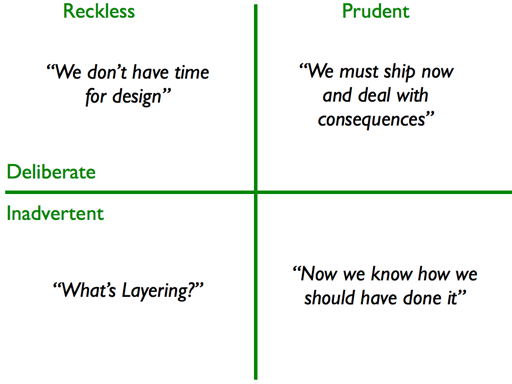
\includegraphics[width=0.5\columnwidth]{images/introduction/technical_debt_quadrant}
	\caption{The technical debt quadrant, as proposed by Martin Fowler.}
	\label{fig:technical-debt-quadrant}
\end{figure}

Technical debt has several interesting properties, explored and defined in the work of Brown et al\cite{brown2010managing}. 
Whether the debt is visible or not is an important factor during software engineering as significant problems can arise when the debt is not clearly visible to other developers.
The value of technical debt is the economic difference between the system as it is and the system in an ideal state for the assumed environment.
The technical debt is relative to a given or assumed environment.
The phenomena has an origin which can be traced back to strategic decisions taken earlier in the development process. Otherwise, the debt could be accumulated in a more unintentional way, either due to recklessness or a lack of knowledge.
Finally, we consider the impact of the technical debt: for instance, what are the required changes we have to perform in order to pay off the debt?\\\\
From the perspective of end users, technical debt can be both invisible and visible\cite{kruchten2012technical}.
Examples of invisible technical debt includes code smells, coding style violations, low internal quality and high code complexity, issues developers should deal with.
Visible debt is expressed in defects that are affecting users but can also be identified by user-unfriendly, cluttered Graphical User Interfaces (GUIs) that has been subject to various reckless modifications: decisions to extend and evolve the user interface with new visual elements, can lead to a high amount of technical debt and a poor user experience.
In more extreme cases, the price of technical debt has to be paid with human lives as is painfully illustrated by a Toyota car accident due to unintended acceleration: after a review of Toyota’s software engineering process and the source code for the 2005 Toyota Camry car, it was concluded that the system was defective and dangerous, riddled with bugs and gaps in its failsafes that led to the root cause of the crash\cite{toyotatechnicaldebt}.\\\\
The term itself is borrowed from the finance domain\cite{guo2011portfolio}.
There is however one important distinction between financial debt and technical debt: when dealing with financial debt, the costs that the debtor has to pay is usually clear.
This is not always the case with technical debt since there might be some situations where no technical debt is incurred.
For instance, if it is known for a part of the system to never be updated or maintained in the future, development time and budget can be saved by not updating the related documentation.
Software engineers need to be carefully with the consideration what technical debt they wish to incur and when this debt will be paid off at specific points in time.\\\\
There are several causes that contribute to the amount of accumulated technical debt during the software development process\cite{martini2014architecture}. Time pressure can cause developers to think reckless about their design and architecture. Uncertainty in decision making during an early stage of development might lead to higher technical debt later on. Finally, in an agile environment, software requirements might change more often, causing the underlying architecture and code base to change to a certain extent. Not properly managing such changes can lead to significant technical debt.\\\\
Technical debt often becomes a noticeable problem in large systems that are built and maintained by many contributors. Tribler is an example of such a system: the software is the result of ten ongoing years of scientific research in the area of decentralized network technology and has incurred a serious amount of technical debt, both visible and invisible for users.
The software is the combination of four disruptive techniques in one large code base: \emph{BitTorrent}, allowing users to download files in a decentralized matter, \emph{Tor}, providing anonymity and strong encryption, \emph{Bitcoin}, offering a way to introduce the notion of trustworthiness inside a decentralized network and \emph{Wikipedia}, allowing collaborative editing of content. These components are depicted in Figure \ref{fig:tribler-connections}.\\

\begin{figure}[t]
	\centering
	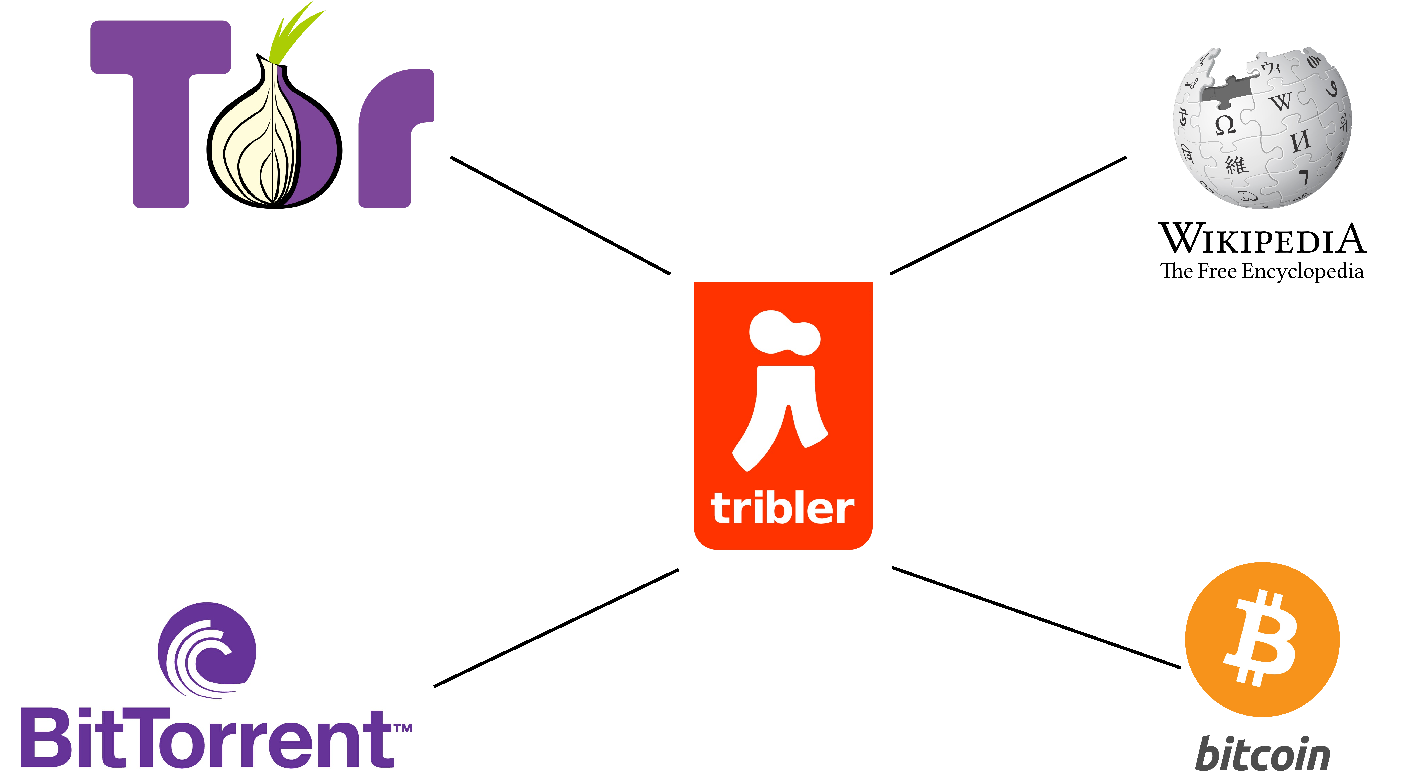
\includegraphics[width=0.6\columnwidth]{images/introduction/tribler_connections}
	\caption{The four disruptive technologies as integrated in Tribler.}
	\label{fig:tribler-connections}
\end{figure}

Anonymity by the utilization of a Tor-like protocol has been added In 2014 by the work of R. Plak\cite{plak2014anonymous} and J.H. Tanaskoski\cite{tanaskoski2014anonymous}. 
In 2015, the protocol has been extended to support anonymous seeding of torrents\cite{ruigrok2015bittorrent}.
The graphical user interface of Tribler is shown in figure \ref{fig:tribler-interface}.

\begin{figure}[!h]
	\centering
	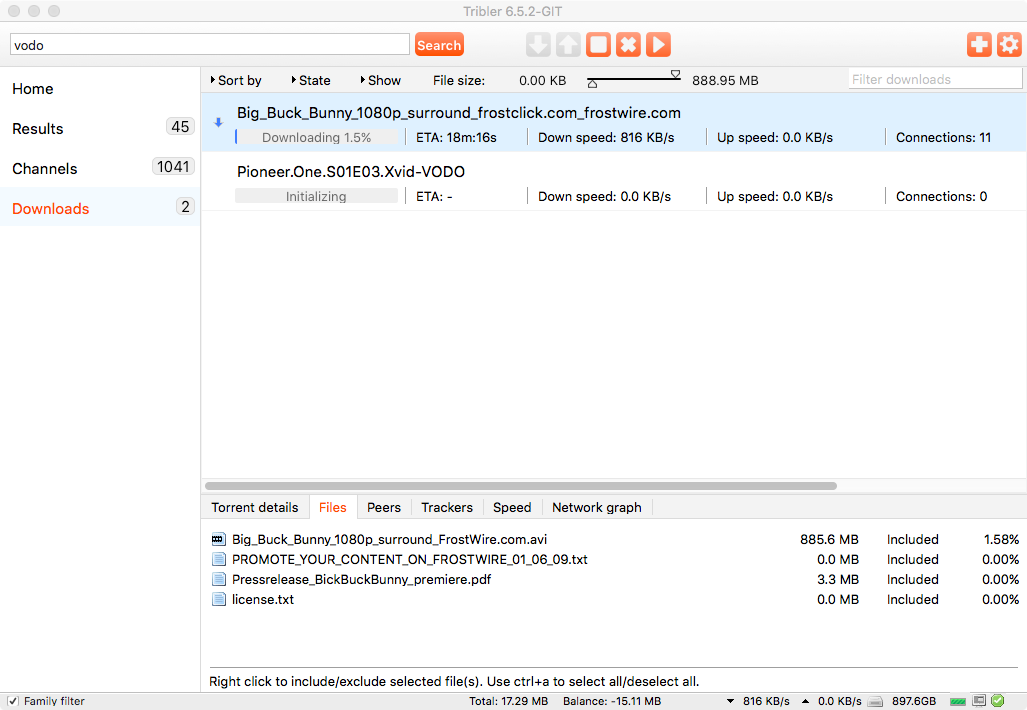
\includegraphics[width=0.9\columnwidth]{images/introduction/tribler_interface}
	\caption{The graphical user interface of Tribler v6.5.2.}
	\label{fig:tribler-interface}
\end{figure}

This thesis work will be centred around identification and management of the accumulated technical debt within the code base of Tribler. With this in mind, we can be formulated the following research question:\\\\
\emph{How can we track, manage and prevent technical debt within Tribler?}\\\\
This question can be divided into several sub questions:
\begin{enumerate}
	\item What are the adequate tools to identity the amount of technical debt within Tribler?
	\item What is the right approach to pay off each identified kind of technical debt?
	\item What are the adequate requirements in the software development process to prevent decisions that are leading to a high amount of debt later in the development process?
\end{enumerate}
The rest of this document is outlined as follows: in Chapter \ref{chapter:problem-description}, the current state of the system will be elaborated, highlighting flaws and impurity in the design and code base. 
In Chapter \ref{chapter:architecture}, the evolution of Tribler over the past ten years will be presented and we lay the foundations for a next decade of scientific research with Tribler by proposing a new future-proof and robust architecture.
The first efforts towards a realisation of this new architecture will be discussed in Chapter \ref{chapter:towards-new-architecture} by the implementation of a RESTful API and a new user interface. Next, in Chapter \ref{chapter:refactoring}, we will focus on the question whether we should pay off the debt in the core of Tribler and how we can do that. 
We will discuss efforts to improve code quality, architecture, infrastructure and the testing framework.
The performance of Tribler after our refactoring efforts will be discussed in Chapter \ref{chapter:experiments}.
By conduction various benchmarks and performance measurements, the user experience of Tribler will be assessed.
We will end with the conclusions and propose future work in Chapter \ref{chapter:conclusions}.
